\subsubsection{The Titan supercomputer}
\label{sec-experiments-1-1}

One of the supercomputers that we consider as a use case for modeling allocation utilization is Titan that is located at the Oak Ridge Leadership Computing Facility (OLCF) in the Oak Ridge National Laboratory (USA). Titan\footnote{The Titan supercomputer, \url{https://www.olcf.ornl.gov/olcf-resources/compute-systems/titan/} [accessed on 2020-02-10]} is a hybrid-architecture Cray XK7 system that contains both CPUs (16-core AMD Opteron) and GPUs (NVIDIA Kepler). It features 18,688 compute nodes, a total system memory of 710 TB, and Cray's high-performance Gemini network. Titan's theoretical peak performance exceeding 27 petaFLOPS.

The general overview of jobs processing at the Titan supercomputer is presented by the following plots (Figures~\ref{fig-titan-logs-waiting-time},~\ref{fig-titan-logs-execution-time}) that demonstrate metrics such as waiting and execution times, as well as requested and eventually used nodes per job (Figure~\ref{fig-titan-logs-nodes-count}) during the defined period of time.

Quantitative characteristics of the presented plots are the following:
\begin{itemize}
    \item waiting time (hours): mean=6.21, std=29.77
    \item execution time (hours): mean=0.61, std=1.51
    \item number of nodes per job: mean=135.07, std=712.31
\end{itemize}
These numbers give a general overview of jobs key characteristics while processing at the Titan supercomputer, and which are compared with the results of simulation runs (outcome of the simulator).

\begin{figure}
    \centering
    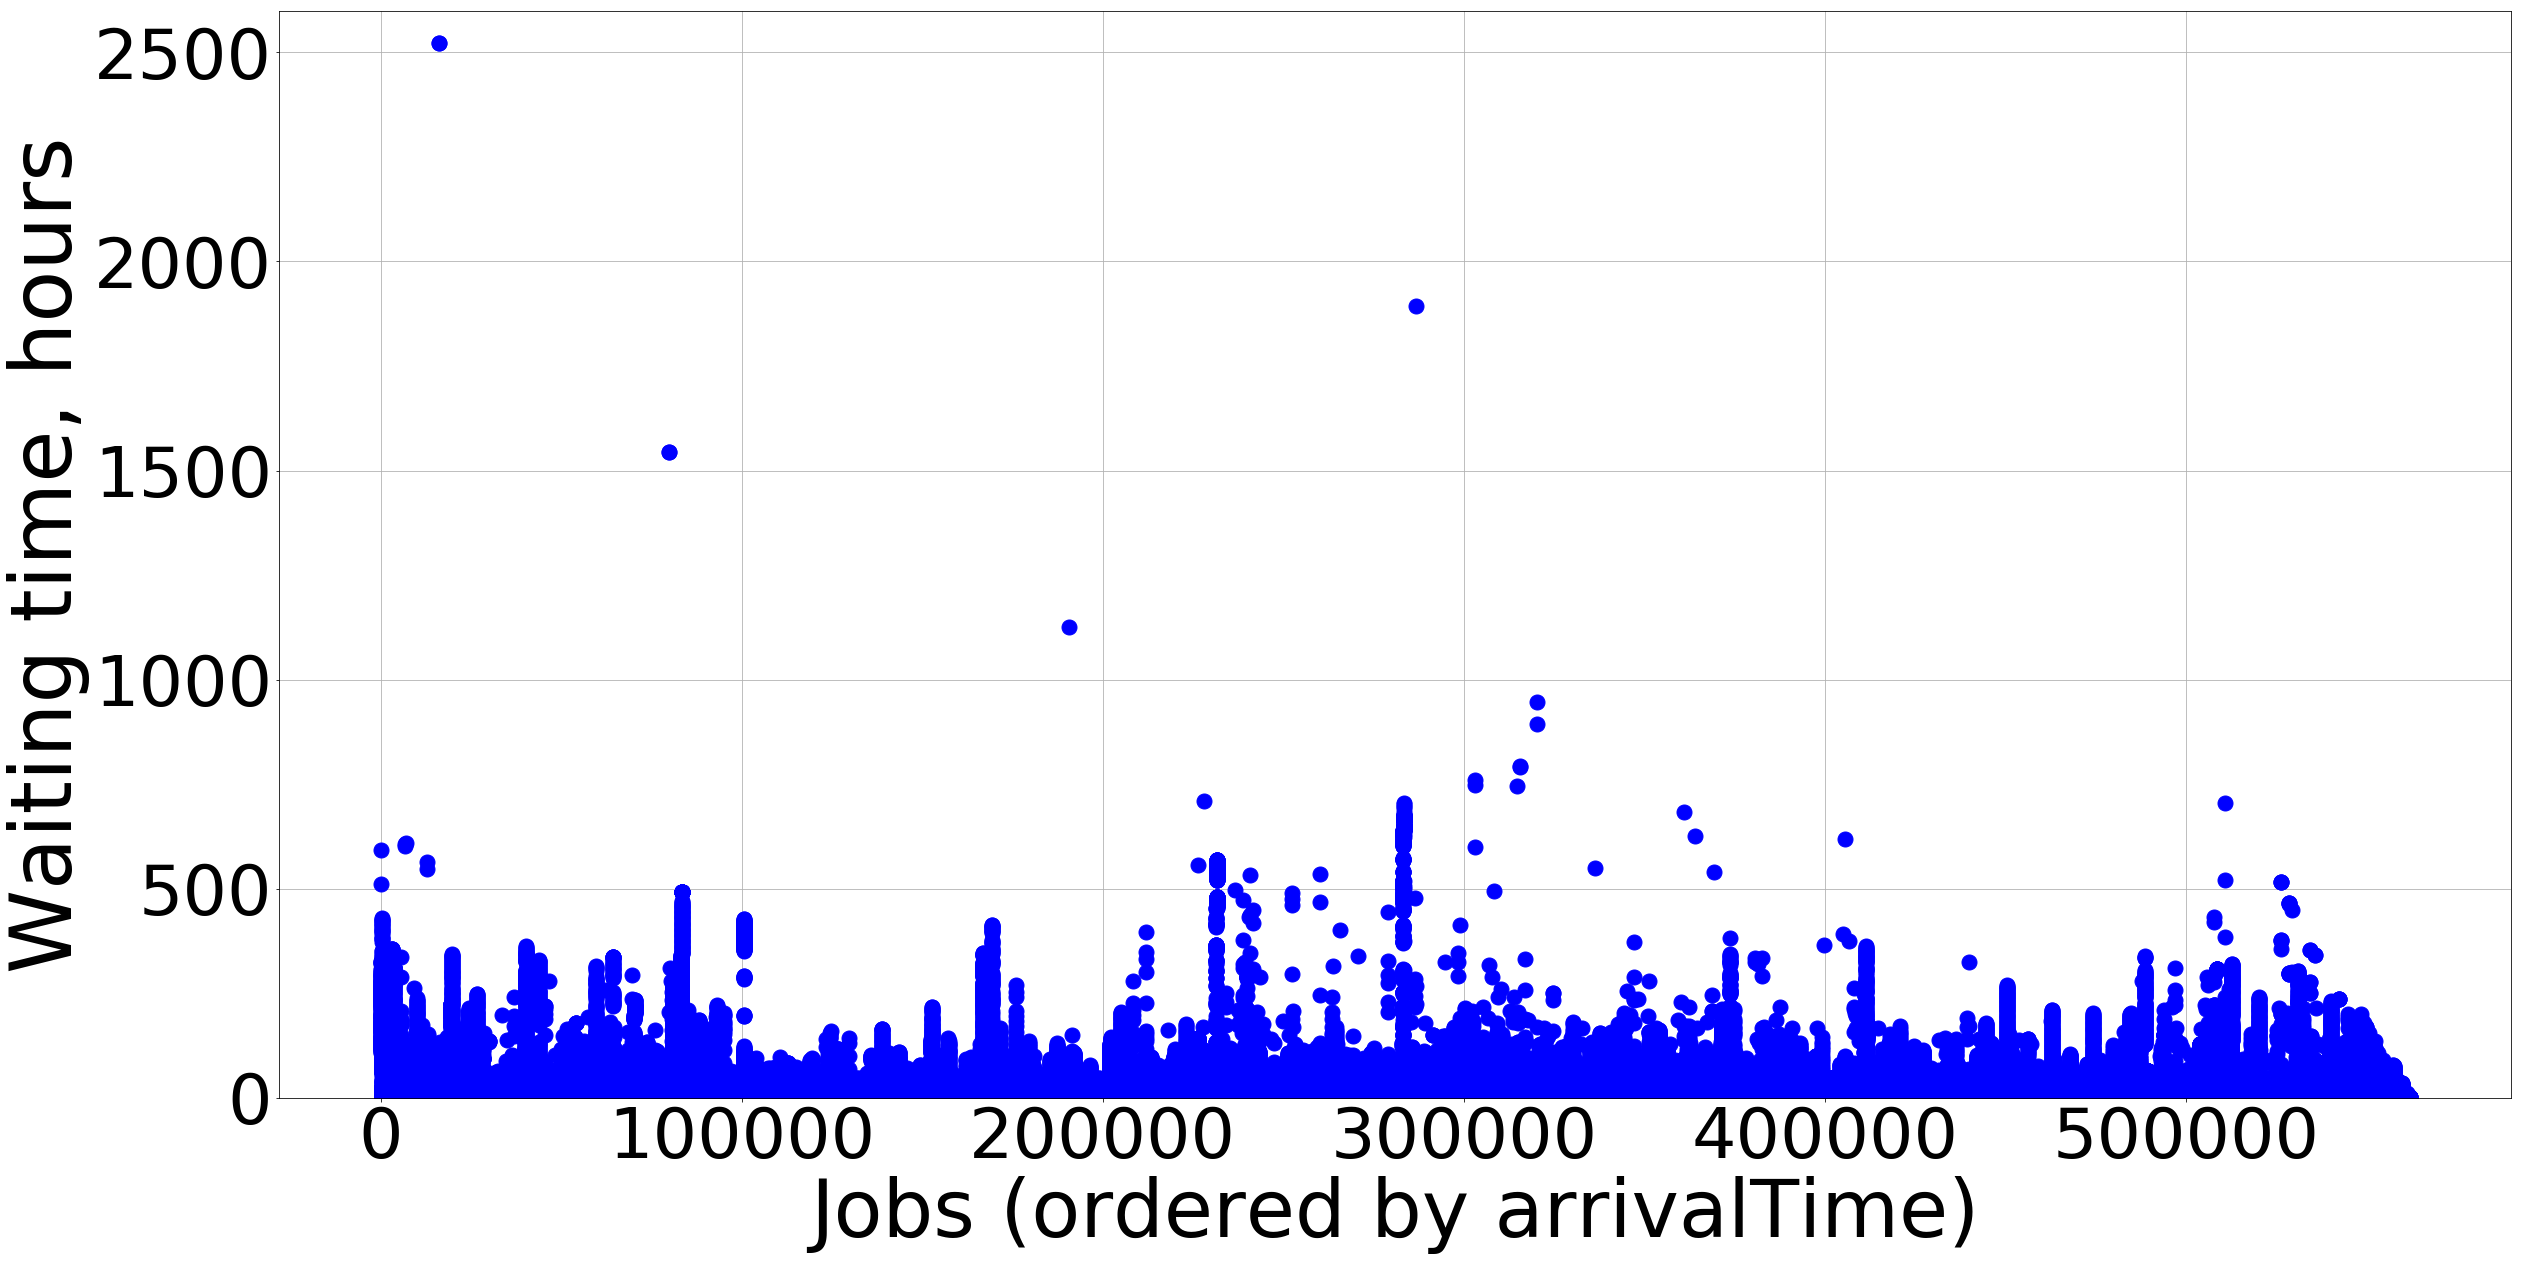
\includegraphics[width=0.45\textwidth]{pics/titan-logs-waiting-time.png}
    \caption{Waiting times for jobs in the queue at the Titan supercomputer (562,079 computing jobs from May 2017 to April 2018)}
    \label{fig-titan-logs-waiting-time} 
\end{figure}

\begin{figure}
    \centering
    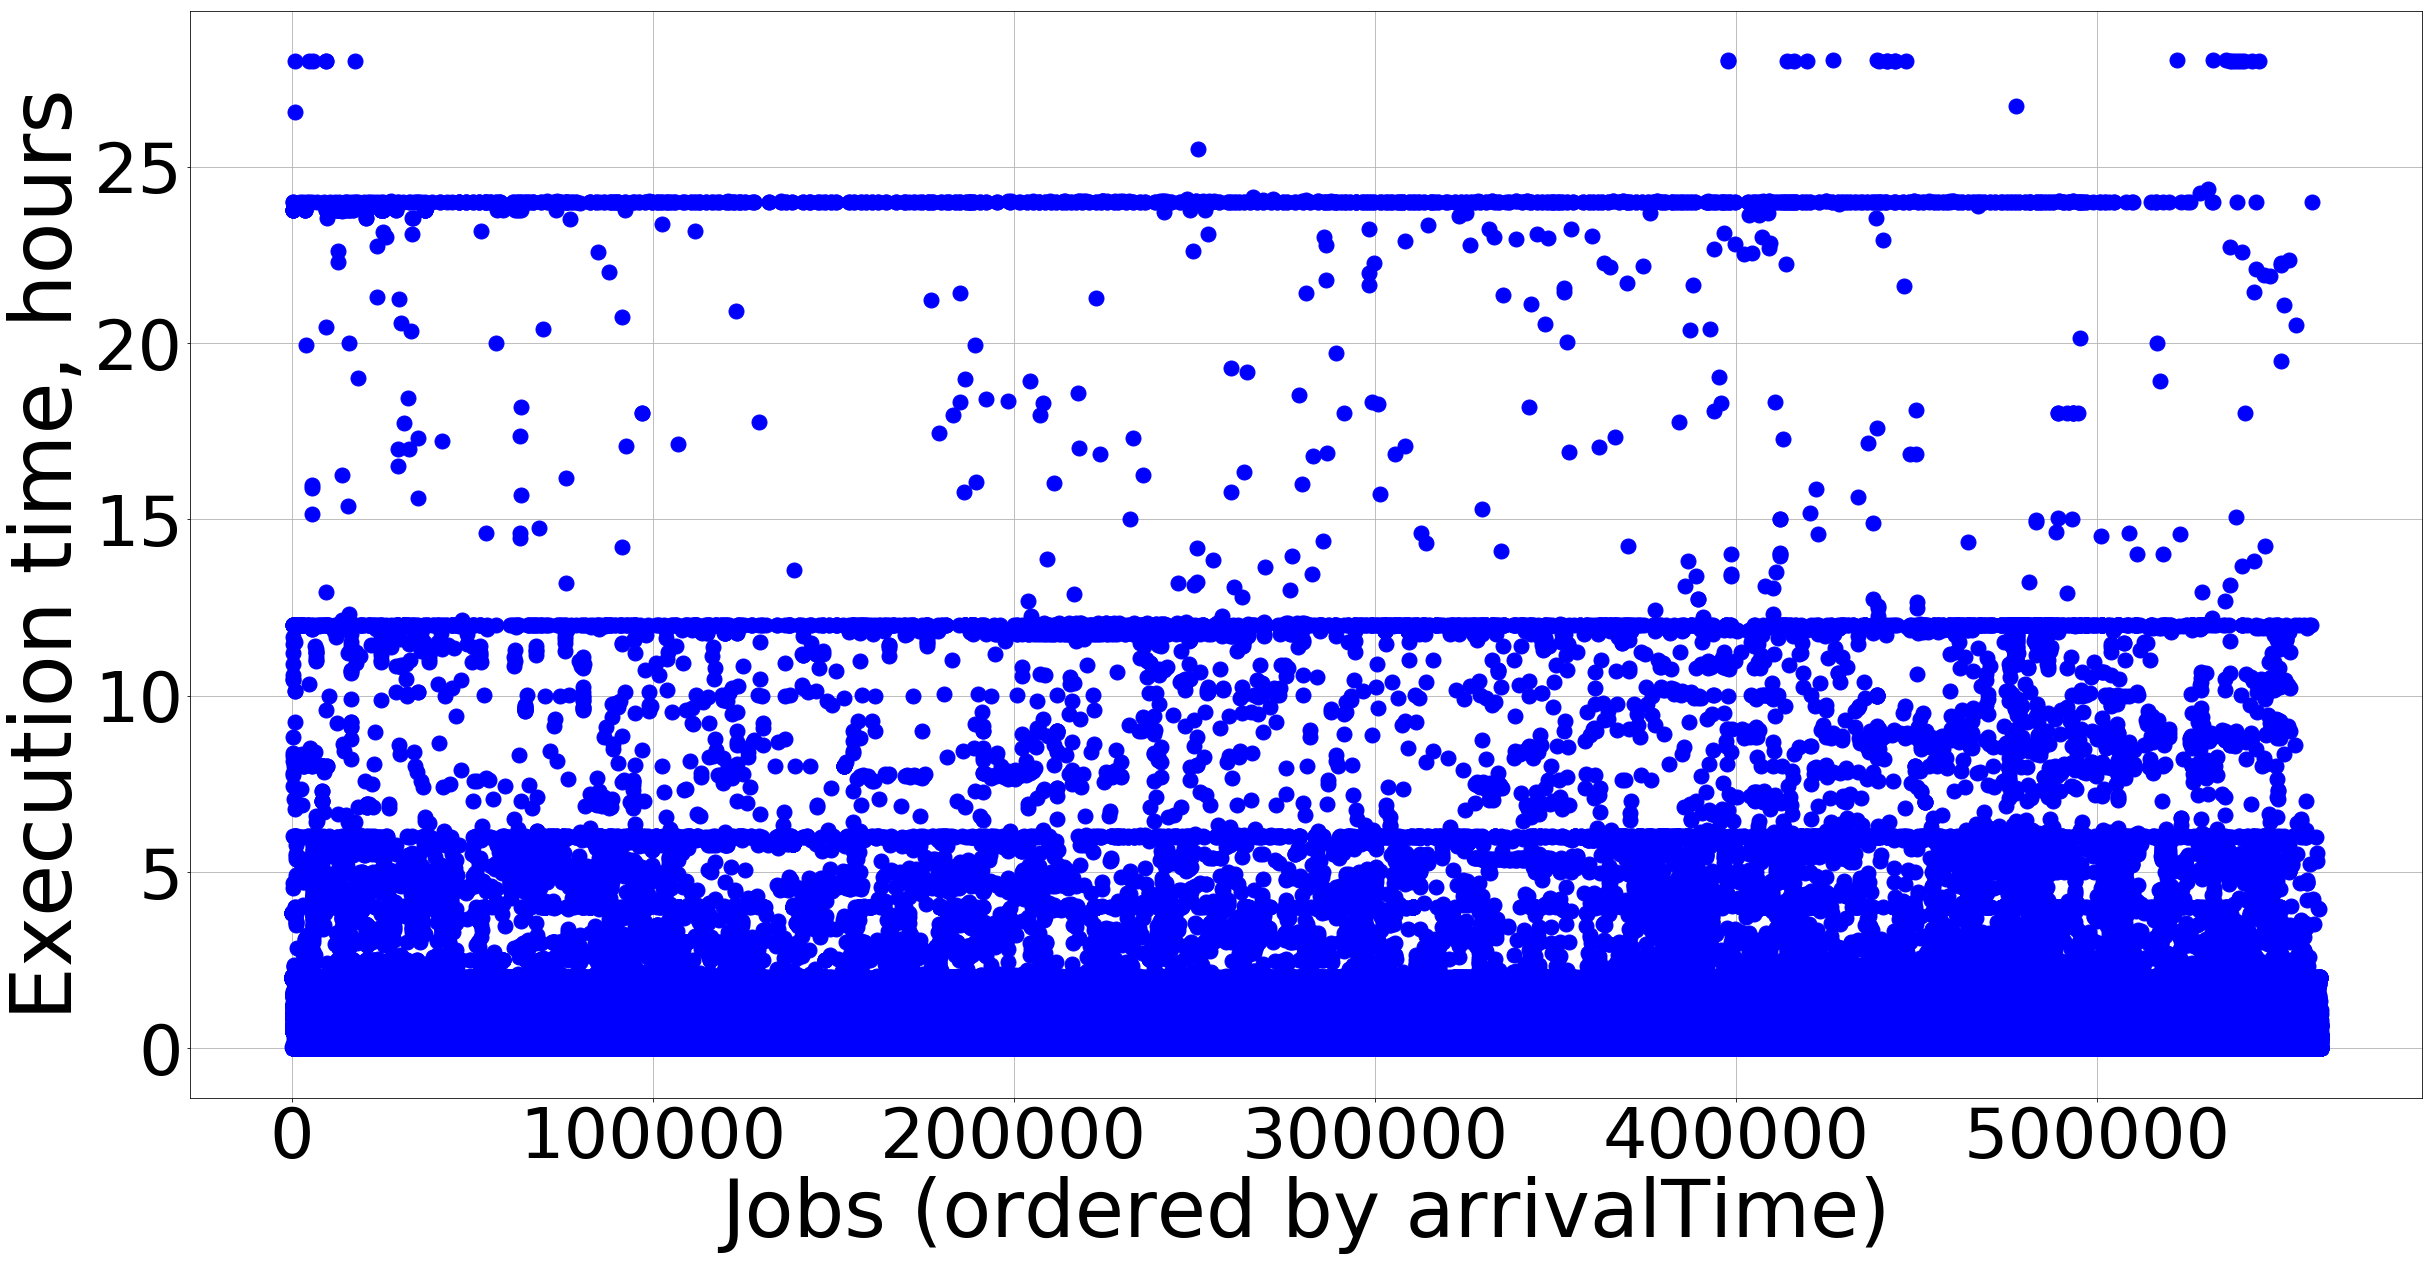
\includegraphics[width=0.45\textwidth]{pics/titan-logs-execution-time.png}
    \caption{Execution times for jobs processing at the Titan supercomputer (562,079 computing jobs from May 2017 to April 2018)}
    \label{fig-titan-logs-execution-time} 
\end{figure}

\begin{figure}
    \centering
    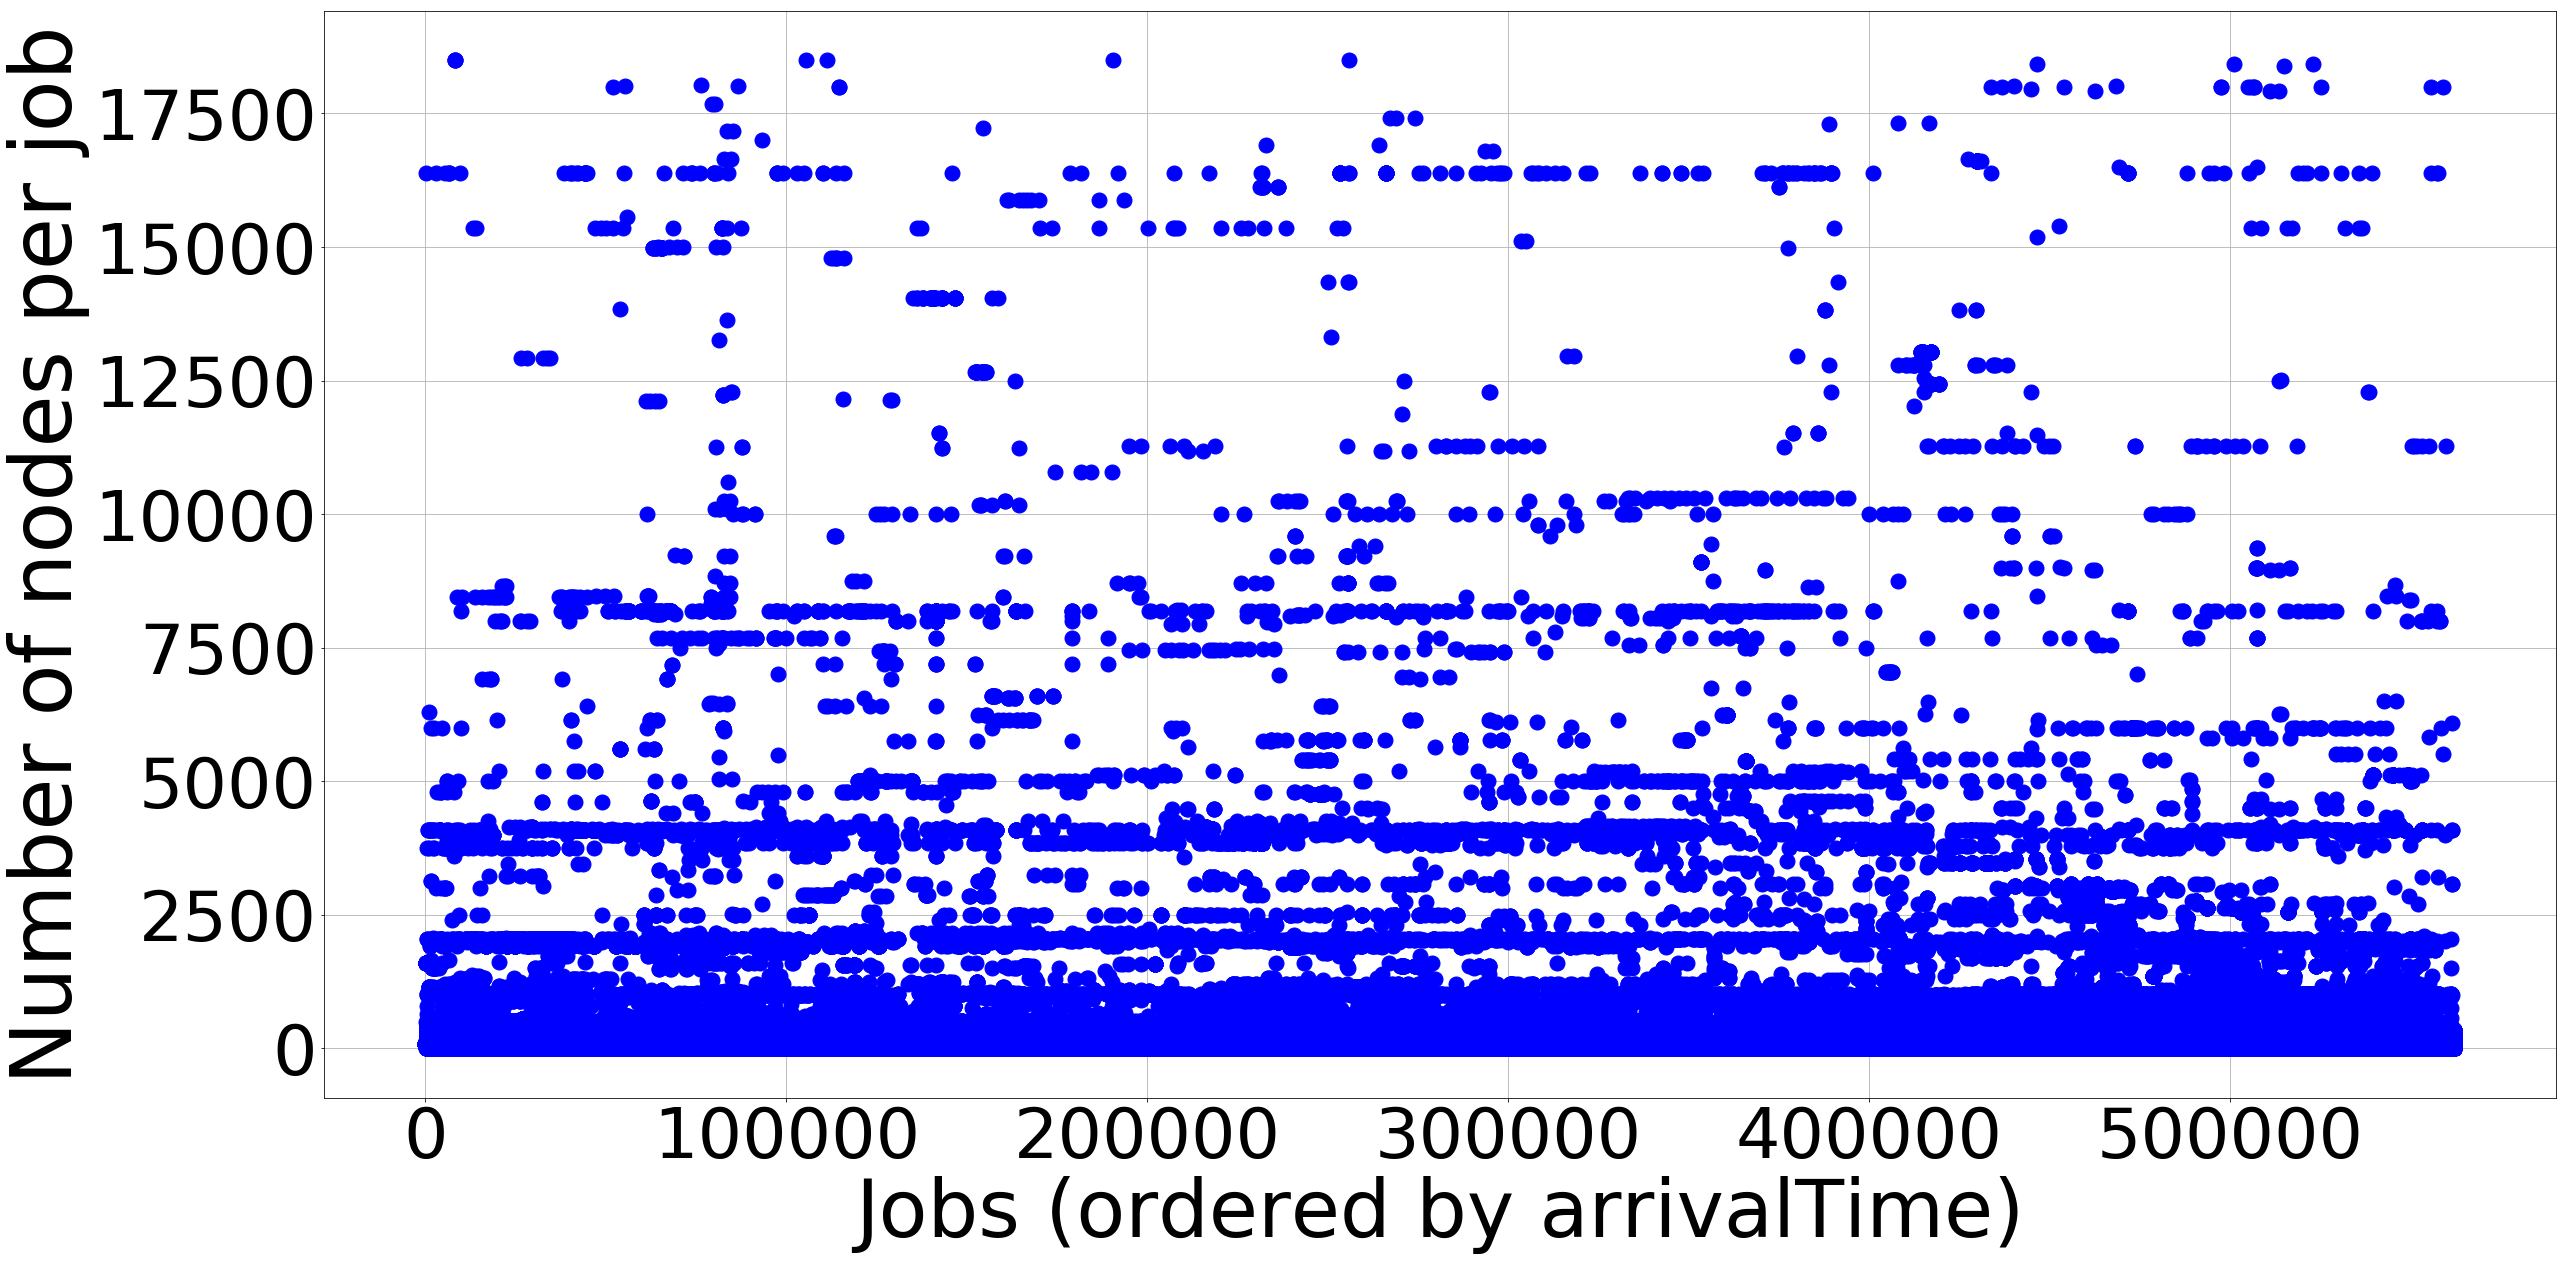
\includegraphics[width=0.45\textwidth]{pics/titan-logs-nodes-count.png}
    \caption{Number of nodes per job at the Titan supercomputer (562,079 computing jobs from May 2017 to April 2018)}
    \label{fig-titan-logs-nodes-count} 
\end{figure}

\subsubsection{Production and Distributed Analysis system PanDA} \label{sec-experiments-1-2}

The PanDA (Production and Distributed Analysis) system is a workload management system (WMS) for job scheduling on the distributed computational infrastructure~\cite{ref-panda}, it federates hundreds of heterogeneous computing resources (including Grid, supercomputers, and public and private computing clouds) into a unique job submission system. It was originally developed for US physicists and adopted as the ATLAS~\cite{ref-atlas} wide WMS in 2008 (in use for all computing applications of the ATLAS experiment at the Large Hadron Collider).

Key features of PanDA are the following: i) pilot-based job execution system with late binding (i.e., there is a lightweight process scheduled on computing nodes that interacts with the core to schedule computing jobs); ii) central job queue; iii) fair-share or policy driven priorities for thousands of users and hundreds of resources; iv) automated brokerage based on CPU and storage resources.

PanDA started to use the Titan supercomputer as one of its resources several years ago under the project of integration with it by enhancing with tools and methods relevant to work on HPC~\cite{ref-titan-prodsys}. Thus, the pilot runs on Titan's data transfer nodes (DTNs) and submits corresponding payloads to the worker nodes. It uses the local job scheduling and management system (Moab) via the SAGA (Simple API for Grid Applications) interface~\cite{ref-saga} for monitoring and management of PanDA jobs running on Titan's worker nodes.

In 2017, under the ALCC\footnote{ALCC: the ASCR (Advanced Scientific Computing Research) Leadership Computing Challenge, \url{https://www.energy.gov/science/ascr/advanced-scientific-computing-research} [accessed on 2020-02-10]} program it was allocated computational resources ($cores \times hours$, i.e., computing hours) at the OLCF supercomputer Titan for ATLAS payload via PanDA.
